\documentclass{article}

\usepackage{fancyhdr}
\usepackage{amsmath}
\usepackage{amsfonts}
\usepackage{bm}
\usepackage[margin=1in]{geometry}
\usepackage{verbatim}
\usepackage{graphicx}

\pagestyle{fancy}

\newcommand{\enum}[1]{\begin{enumerate}#1\end{enumerate}}

\title{Network Equilibria: An Applied Approach}
\author{Moya Chen \and Louis O'Bryan \and Victor Duan}


\begin{document}
\begin{titlepage}
    \maketitle
    \vfill
    \begin{center}
        {\large CS 143 Communication Networks \\ Final Project, Fall Term 2013}
    \end{center}
    \vfill
    \thispagestyle{empty}
\end{titlepage}

\tableofcontents
\newpage

\section{Introduction}
Networking theory is an important part to the function of the Internet. Congestion control algorithms can heavily influence the speed of a connection. 

In this paper, we describe the implementation of a network simulator including its architecture and design choices. We also include graphs of this simulator as run on a series of test cases. Lastly, we give a mathematical analysis for one of the congestion algorithms, as applied to one of the cases.

\section{Simulator Description}
    Our network simulator is written in C++. 
    
    The network consists of several different types of network classes as well as a Controller to monitor the simulation. 
    
    We use event-based simulation, with a global event queue, to advance actions in our program. 
    
    For input, we take an XML file as input and use the pugixml C++ XML parser to read the file and create necessary network objects. The program uses these objects to simulate the network until all the flows finish. 
    
    The congestion control algorithms we implemented were TCP Reno and TCP Vegas.

     As the simulation runs, we collect various statistics. At the end of the simulation, we use gnuplot to create figures based off of collected data.

\subsection{Design Decisions}
    We chose to write the simulator in C++ for several reasons. C++ is a powerful and fast object oriented programming language which suited our architecture plan well. We wrote classes for different network objects (Link, Flow, etc.) as well as simulation objects (Controller, CongestionAlgorithm, etc.). By using C++’s inheritance, we were able to group objects with similar behavior (ex. Host and Router) and create abstraction hierarchies (ex. Node, Packet).  C++ allowed for writing these classes with encapsulation.

    Because the network that we are simulating is based on discrete events, we chose to use event-based simulation. Continuous simulation did not make sense as it would be very CPU heavy and take a longer time to run on our computers. Because we knew that we would be spending a fair amount of time running code, we figured that event-based simulation would be the most efficient.

    We chose the pugixml parser because it is lightweight and has a simple, open-source library. The lightweightness was particularly attractive because we did not want the simulator to be spending most of its runtime parsing input files. Furthermore, the pugixml library was easy to use. XML was the chosen input format because as a universally recognized format it was easy to make it fit our desired system parameters. Thus, we ended up using an XML DOM type input, as it could easily describe the objects we wanted for the simulation.

    We chose two TCP congestion control algorithms: TCP Reno and TCP Vegas. We wanted to choose one loss-based congestion control algorithm (Reno) and one delay-based congestion control algorithm (Vegas). We chose Reno because among the loss-based control algorithms (Reno and Tahoe) because it included more advanced congestion control through the use of fast\_recover. Further equations for the analysis are in the notes. Obviously, this section needs some work/deleting.
    Maybe a paragraph on why we chose gnuplot.


\begin{figure}[htbp]
    \centering
    \includesvg[width=0.5\textwidth]
    {reno2/Flow_Recieve_Rates.svg}
    \caption{ ... caption text ... }
\end{figure}
\begin{comment}
/Flow_Outstanding_Packets.svg
/Flow_Recieve_Rates.svg
/Flow_RTT.svg
/Flow_Send_Rates.svg
/Flow_Window.svg
/Host_Receive.svg
/Host_Send.svg
/Link_Flow_Rate.svg
/Link_Occupancy.svg
/Link_Packet_Loss.svg
/Vegas_Diff.svg
\end{comment}







% !TEX root = Report.tex


\section{Architecture}

    The network design was split into the groups of classes as follows: Simulation, Network, and Input. The Simulation group contains the classes Event, Scheduler, and Controller. These classes are used to hold the network objects as well as manage the event-based simulation. The Network group contains the classes Node, Host, Router, Link, Buffer, Router, RoutingTable, Packet, RoutingPacket, RouterRoutingPacket, HostRoutingPacket, DataPacket, AckPacket, Flow, CongestionAlgorithm, SLOW\_START, TCP\_TAHOE, TCP\_RENO, Vegas, and Cubic. These classes are used to simulate network objects and their behavior. Their exact behavior and hierarchy are described in more detail below. Finally, the Input group of classes contains InputParser, SystemInfo, HostInfo, RouterInfo, LinkInfo, and FlowInfo. The InputParser is used to read in information from the input XML file and that information is used in Controller to create the objects.

\subsection{Simulation Classes}
    Classes in this category: Controller, Scheduler, Event

    The Simulation classes function to keep track of high-level system parameters as the simulation runs. 
The Controller class has a few main tasks. One instance of this class is created upon program start. (For simplicity, we will refer to this one instance of the Controller class as “the controller”.) It is the Controller to which the InputParser adds system objects. (See Input/Output below.) The controller is what keeps track of system time. It also contains an instance of Scheduler (hence forth called “the scheduler”). It is also the object that interfaces with network objects when the network objects want to make events. The controller also initializes the first routing update and system print events. After initialization, these Events will schedule the next instance of themsleves.

 In essence, the controller runs the entire simulation.

The scheduler contains a priority queue, ordered by event time, which contains all of the system’s events. In this scheduler, there is a doNext() function which is called by the controller until the system has finished running of all of its flows. This function enacts the next event in the queue. 

The Event class contains 3 things: a timestamp for when the event should be executed, a function pointer to the function scheduled, and a pointer to arguments that the function may need for execution. When an Event is executed, the function is called with the arguments.

    To do event-based simulation, each element in the system that wants to call some function in the future will create a new Event with the time of execution, the function, and appropriate arguments. It will then call the controller's add(Event *e) function in order to put this new Event into the scheduler's queue. Until the simulation finishes, the controller pops off the top Event off of the scheduler queue, executing it. It then checks if there are any flows left. If there still exist flows, it pops the top Even off of the scheduler queue again, and so on and so forth. 

    In order to make sure that periodic events like router updates and system snapshot happen, the controller is initialized with the first Event of these. For system snapshot, the controller iterates through all links, routers, hosts, and flows, writing appropriate data to output files and resetting necessary statistics. Router updates trigger the creation of routing packets at each router, which are put into the different links. When these packets are recieved by routers and hosts, they create packets as appropriate, sending them back to the routers which are used for updates.  



\subsection{Network Classes}

\begin{figure}[htbp]
    \centering
    \includegraphics[width=0.5\textwidth]{hierarchy.png}
    \caption{An image of hierarchy of network object classes in our system. Arrows denote inheritance. Boxes inside of boxes denote a single instance of an object of a class being initiated as part of every instance of another class. (Ex. a link always contains 2 buffers)}
\end{figure}

    The Network classes are used to hold information of the various network objects. They are split into a few general subgroups: Node, Link, Packet. Node is further split into Host and Routing. Because Host and Routing is fairly involved, we will explain these in detail as well. 

    \paragraph{Node} The Node subgroup consists of Node, Host, and Router. Node is an abstract class that contains the id of the node as well as the list of links to which is connected. The Node class guarantees a function handlePacket(Packet *p). We choose to implement this abstract class because class Router and Host both have this as part of their interface. 
    
    \paragraph{Router} The Routing subsubgroup consists of Router and RoutingTable. Each router contains its own RoutingTable pointer which describes the behavior it will follow when routing packets. The RoutingTable itself is a map from Node pointers to pairs of weight and Link pointers. The key is the destination Node of the packet to route. It is a Node (as opposed to Host) because while all DataPackets must be sent to Hosts, RoutingPackets can also be sent to Routers. The weights are then the weight of that path and the Link is the next link to follow on that path. In addition to the routing table, the primary function of the Router class is to handle packets that it receives. Data and ack packets are simply forwarded to the next link in the path. Routing packets, on the other hand, are used to update the router’s own routing table. This is done in the routing table update steps every routingTableUpdateTime. 

As far as the actual routing updates are done, we implement the Bellman-Ford algorithm. We chose to use this algorithm because it utilizes local knowledge of the graph as opposed to Dijkstra’s algorithm, which depends on global knowledge of the network. As such, it seems more natural to use Bellman-Ford for the routing table updates. Dynamic routing is calculated through a combination of buffer delay and propagation delay. Buffer weights are only calculated once per routing update period so that the routing table weights -- stored as doubles -- stabilize. This behavior mimics real routing table updates because otherwise the routing weights constantly change by slight amounts.

    \paragraph{Host} The Host subsubgroup consists of the Host class, the Flow class, as well as all of the congestion control algorithm classes. These classes together are responsible for the creation and tracking of data and acknowledgement packets sent throughout the system.
    
    The Host class is responsible for data collection and passing packets from Links to Flows. 
    
    The Flow class holds onto the information needed to handle the flow, including size, progress, outstanding packets, acks received, and relevant stat fields. Flows also include an instance of CongestionAlgorithm. The Flows create DataPackets upon request from the CongestionAlgorithm, which it sends to its source Host for transfer. When a DataPacket is received by the recieve Host, the Flow keeps track of which id it should use to create an AckPacket for in response to the reception of that DataPacket. When a Flow is added to the Controller, an initial event is scheduled to cause the first data packet transmission. 
    
    CongestionAlgorithm is the abstract base class used to simulate the congestion control algorithms. It holds onto fields necessary for congestion control such as window size and ssthresh. We then have several different congestion control algorithms that implement various types of TCP congestion control. 
    
    The simplest of these is SLOW\_START, which inherits from CongestionAlgorithm. SLOW\_START implements slow start for that part of TCP, and then uses very basic congestion avoidance. While not in slow start, it increments cwnd by 1/cwnd every ack. Otherwise, it increments cwnd by 1. When packets time out, it sets ssthresh to half cwnd and sets cwnd to 1. With SLOW\_START, it is possible to see network behavior while running just only multiplictive increase and congestion avoidance. 
    
    Next, we have TCP\_TAHOE, which inherits from SLOW\_START. TCP\_TAHOE implements fast\_retransmit. In fast\_retransmit, when 3 duplicate ACKs are recieved, it is treated the same as a timeout. Rather than having to wait a full round trip time in order to send a new packet, TCP\_TAHOE detects packets sooner than SLOW\_START. Thus, we can implement Additive Increase, Multiplicative Decrease efficiently. 
    
    After this, we have TCP\_RENO, which then inherits from TCP\_TAHOE. This adds fast\_recovery. Rather than sending a single packet upon detecting packet loss from triple acknowledgement, TCP\_RENO includes a modified algorithm which temporarily inflates the window size to compensate for packets as they go missing. Thus, rather than collapsing the window size to 1 as soon as packet loss is detected, TCP\_RENO can adjust to a more reasonable size and adjust from there. 
    
    We also have Vegas, which inherits from TCP\_RENO. The Vegas algorithm is very similar to TCP\_RENO except that it has a different window update rule in Congestion Avoidance. Rather than using packet loss as its main metric, it uses packet delay. This allows more fine-grained tuning of network status as packets are being sent and recieved. The idea of Vegas is that there is some ideal range for the value of the current window size divided by what the round trip time would be of the system if there were no queuing delays compared to if there were. By keeping this difference within a constant set of values, we can ensure that window size is not too big or not too small. 
    
    Finally, we have Cubic, which inherits from SLOW\_START. It is a TCP algorithm based on a window update algorithm using a Cubic function. While this class currently does not currently run successfully on simulation, we have included it nonetheless for possible future work. 
    

    \paragraph{Link} The Link subgroup consists of Link and Buffer. The Buffer class is used to simulate the buffers on the links. Each link has two buffers, one in each direction and each have the capacity described in the input file. It also consists of pointers to the Nodes to which an instance of Link is attached.
    
    The buffers are implemented as FIFO queues of Packets. The Link class uses the buffers and its own fields to manage the link’s activities. 

    The Link also includes various functions to handle packet transfer. We describe them in the section Packet Transfer below. 

    \paragraph{Packet} The Packet subgroup consists of the large variety of Packet classes. All of these stem from the abstract Packet class. Packet contains core information of the packet such as id, size, source, and destination, and packet type. 
    
    There are two subgroups of Packets: RoutingPacket and Datapacket. 
    
    Inheriting from Packet, we have RoutingPacket, which are the packets used to update the Router's RoutingTables. In class RoutingPacket, we add a field to describe the link that a RoutingPacket packet came from. 
    Inheriting from RoutingPacket, we have RouterRoutingPacket and HostRoutingPacket. HostRoutingPackets tell Routers that the hosts still exist at that link. RouterRoutingPackets contain routing tables to tell the routers whether or not they have to update their routing tables. 
    
    In class DataPacket, we inherit from Packet. Data packets use extra information for the flow it is part of and the start time, which is used for calculating stats such as RTT and packet delay. Finally, we have AckPacket, which inherits from DataPacket. We inherit from AckPacket as many of the properties (such as flow) are the same between the two. This also aids in debugging, as we can print which DataPacket triggered the creation of which AckPacket. DataPacket and AckPacket are both created by the Flow. 


\subsubsection{Packet Transfer}    
\begin{figure}[htbp]
    \centering
    \includegraphics[width=\textwidth]{packetTransfer.png}
    \caption{Packet transfer process between nodes (hosts, routers) and links. Arrows here represent packet transfer in the system. Arrowhead direction denotes passing of packets between functions. Arrow label denotes time offset added, as perceived by scheduler. (Time offset is zero when not labeled.) }
\end{figure}

Because the packet transfer structure may be a bit confusing without explaination, we provide one here.

When a node puts a packet into the link, it will call that link's handlePacket(Packet *p) function. Because there may be other packets traveling the link at the same time, we first schedule an event which calls sendAnotherPacket on the link. This event is scheduled at a time so that delays that may be incurred at the head of a link (queue delay, processing delay) are included.

When sendAnotherPacket is called, we schedule an event that calls sendPacketCallback. This simulates the delay time that a link would have in transmitting the packet over its length. 

Finally, when sendAnotherPacket is called again, we know the packet has finished transmitting the length of the link. Thus, it can be sent on to the next node in the system.  

\subsection{Input/Output}
    The InputParser class uses the pugixml C++ XML parsing ability to parse input files and store the information in lists of the various Info objects. One thing to note is that pugixml does not provide any method of checking the XML file against an XSD schema. As such, the expected input and some behavior is described in much greater detail in the networkSchema.txt file in the InputParser directory.
    
    The SystemInfo class is used as the parent class for the other Info classes. All it holds is the printing flag for the object. The other Info classes each contain values specific to the type of object it is designed to hold information of. For example, LinkInfo will hold members such as linkRate. These are explained in more detail in the networkSchema.txt file.
    
    If the input file is formatted correctly, the InputParser can call its run function, which takes in references to the values it will set, to parse the file, set global parameter fields, and create network objects. The global parameter fields set are snapshotTime, routingUpdateTime, hosts, routers, links, flows, and plotOptions. snapshotTime is the time interval between stat-collecting events. The smaller this is, the finer the resolution. routingUpdateTime is the time interval between updating the routing tables. hosts, routers, links, and flows are lists of their corresponding Info objects that will be used to create the objects later. plotOptions sets various plot settings for gnuplot for the output graphs.
           
\begin{figure}[htbp]
    \centering
    \includegraphics[width=\textwidth]{io.png}
    \caption{Input/output structure of our system. Yellow denotes input/output files. Cyan denotes helper libraries. Blue rectangle denotes simulator objects. Blue diamond denotes simulator events. }
\end{figure}

    System output is done via periodic printing to data files. At the start of the simulation, the controller schedules an event which calls printSystem(). This function iterates through all links, flows, and hosts, requesting and then resetting data as appropriate. This data is written to a series of output files. At the end of the call to printSystem(), the printSystem() function will schedule an event to call itself again at a time snapshotTime later.
    Once the controller has finished running the simulation, it will make a function call to appropriate library functions in gnuplot. This will take the data from the files we have written to above and graph it. 



% !TEX root = Report.tex


\section{Simulator Plots}
In this section, we include the plots resulting from our simulation running on various testcases. 

\newpage
%%%%%%%%%%%%%%%%%%%%%%%%%%%%%%%%%%%%%%%%%%%%%%%%%%%%%%%%%%%%%

\begin{figure}[htbp]
    \centering
    \includegraphics[width=\textwidth]{reno1/Flow_Outstanding_Packets.png}
    \caption{TCP RENO, Case 1: Flow Outstanding Packets}
\end{figure}


\begin{figure}[htbp]
    \centering
    \includegraphics[width=\textwidth]{reno1/Flow_Receive_Rates.png}
    \caption{TCP RENO, Case 1: Flow Receive Rates }
\end{figure}


\begin{figure}[htbp]
    \centering
    \includegraphics[width=\textwidth]{reno1/Flow_RTT.png}
    \caption{TCP RENO, Case 1: Flow Round Trip Time}
\end{figure}

\begin{figure}[htbp]
    \centering
    \includegraphics[width=\textwidth]{reno1/Flow_Send_Rates.png}
    \caption{TCP RENO, Case 1: Flow Send Rates}
\end{figure}

\begin{figure}[htbp]
    \centering
    \includegraphics[width=\textwidth]{reno1/Flow_Window.png}
    \caption{TCP RENO, Case 1: Flow Window}
\end{figure}

\begin{figure}[htbp]
    \centering
    \includegraphics[width=\textwidth]{reno1/Host_Receive.png}
    \caption{TCP RENO, Case 1: Host Receive Rate}
\end{figure}


\begin{figure}[htbp]
    \centering
    \includegraphics[width=\textwidth]{reno1/Host_Send.png}
    \caption{TCP RENO, Case 1: Host Send Rate}
\end{figure}

\begin{figure}[htbp]
    \centering
    \includegraphics[width=\textwidth]{reno1/Host_Send.png}
    \caption{TCP RENO, Case 1: Host Send Rate}
\end{figure}


\begin{figure}[htbp]
    \centering
    \includegraphics[width=\textwidth]{reno1/Link_Flow_Rate.png}
    \caption{TCP RENO, Case 1: Host Send Rate}
\end{figure}

\begin{figure}[htbp]
    \centering
    \includegraphics[width=\textwidth]{reno1/Link_Occupancy.png}
    \caption{TCP RENO, Case 1: Host Send Rate}
\end{figure}

\begin{figure}[htbp]
    \centering
    \includegraphics[width=\textwidth]{reno1/Link_Packet_Loss.png}
    \caption{TCP RENO, Case 1: Host Send Rate}
\end{figure}


\newpage
\clearpage


%%%%%%%%%%%%%%%%%%%%%%%%%%%%%%%%%%%%%%%%%%%%%%%%%%%%%%%%%%%%%%%%%%%

\begin{figure}[htbp]
    \centering
    \includegraphics[width=\textwidth]{vegas1/Flow_Outstanding_Packets.png}
    \caption{TCP VEGAS, Case 1: Flow Outstanding Packets}
\end{figure}

\begin{figure}[htbp]
    \centering
    \includegraphics[width=\textwidth]{vegas1/Flow_Receive_Rates.png}
    \caption{TCP VEGAS, Case 1: Flow Receive Rates }
\end{figure}


\begin{figure}[htbp]
    \centering
    \includegraphics[width=\textwidth]{vegas1/Flow_RTT.png}
    \caption{TCP VEGAS, Case 1: Flow Round Trip Time}
\end{figure}

\begin{figure}[htbp]
    \centering
    \includegraphics[width=\textwidth]{vegas1/Flow_Send_Rates.png}
    \caption{TCP VEGAS, Case 1: Flow Send Rates}
\end{figure}

\begin{figure}[htbp]
    \centering
    \includegraphics[width=\textwidth]{vegas1/Flow_Window.png}
    \caption{TCP VEGAS, Case 1: Flow Window}
\end{figure}

\begin{figure}[htbp]
    \centering
    \includegraphics[width=\textwidth]{vegas1/Host_Receive.png}
    \caption{TCP VEGAS, Case 1: Host Receive Rate}
\end{figure}


\begin{figure}[htbp]
    \centering
    \includegraphics[width=\textwidth]{vegas1/Host_Send.png}
    \caption{TCP VEGAS, Case 1: Host Send Rate}
\end{figure}

\begin{figure}[htbp]
    \centering
    \includegraphics[width=\textwidth]{vegas1/Host_Send.png}
    \caption{TCP VEGAS, Case 1: Host Send Rate}
\end{figure}


\begin{figure}[htbp]
    \centering
    \includegraphics[width=\textwidth]{vegas1/Link_Flow_Rate.png}
    \caption{TCP VEGAS, Case 1: Host Send Rate}
\end{figure}

\begin{figure}[htbp]
    \centering
    \includegraphics[width=\textwidth]{vegas1/Link_Occupancy.png}
    \caption{TCP VEGAS, Case 1: Host Send Rate}
\end{figure}

\begin{figure}[htbp]
    \centering
    \includegraphics[width=\textwidth]{vegas1/Link_Packet_Loss.png}
    \caption{TCP VEGAS, Case 1: Host Send Rate}
\end{figure}

\begin{figure}[htbp]
    \centering
    \includegraphics[width=\textwidth]{vegas1/Vegas_Diff.png}
    \caption{TCP VEGAS, Case 1: Vegas Diff}
\end{figure}

\newpage
\clearpage

%%%%%%%%%%%%%%%%%%%%%%%%%%%%%%%%%%%%%%%%%%%%%%%%%%%%%%%%%%%%%%

\begin{figure}[htbp]
    \centering
    \includegraphics[width=\textwidth]{reno2/Flow_Outstanding_Packets.png}
    \caption{TCP RENO, Case 2: Flow Outstanding Packets}
\end{figure}

\begin{figure}[htbp]
    \centering
    \includegraphics[width=\textwidth]{reno2/Flow_Receive_Rates.png}
    \caption{TCP RENO, Case 2: Flow Receive Rates }
\end{figure}


\begin{figure}[htbp]
    \centering
    \includegraphics[width=\textwidth]{reno2/Flow_RTT.png}
    \caption{TCP RENO, Case 2: Flow Round Trip Time}
\end{figure}

\begin{figure}[htbp]
    \centering
    \includegraphics[width=\textwidth]{reno2/Flow_Send_Rates.png}
    \caption{TCP RENO, Case 2: Flow Send Rates}
\end{figure}

\begin{figure}[htbp]
    \centering
    \includegraphics[width=\textwidth]{reno2/Flow_Window.png}
    \caption{TCP RENO, Case 2: Flow Window}
\end{figure}

\begin{figure}[htbp]
    \centering
    \includegraphics[width=\textwidth]{reno2/Host_Receive.png}
    \caption{TCP RENO, Case 2: Host Receive Rate}
\end{figure}


\begin{figure}[htbp]
    \centering
    \includegraphics[width=\textwidth]{reno2/Host_Send.png}
    \caption{TCP RENO, Case 2: Host Send Rate}
\end{figure}

\begin{figure}[htbp]
    \centering
    \includegraphics[width=\textwidth]{reno2/Host_Send.png}
    \caption{TCP RENO, Case 2: Host Send Rate}
\end{figure}


\begin{figure}[htbp]
    \centering
    \includegraphics[width=\textwidth]{reno2/Link_Flow_Rate.png}
    \caption{TCP RENO, Case 2: Host Send Rate}
\end{figure}

\begin{figure}[htbp]
    \centering
    \includegraphics[width=\textwidth]{reno2/Link_Occupancy.png}
    \caption{TCP RENO, Case 2: Host Send Rate}
\end{figure}

\begin{figure}[htbp]
    \centering
    \includegraphics[width=\textwidth]{reno2/Link_Packet_Loss.png}
    \caption{TCP RENO, Case 2: Host Send Rate}
\end{figure}

%%%%%%%%%%%%%%%%%%%%%%%%%%%%%%%%%%%%%%%%%%%%%%%%%%%%%%%%%%%%%

\newpage
\clearpage


\begin{figure}[htbp]
    \centering
    \includegraphics[width=\textwidth]{vegas2/Flow_Outstanding_Packets.png}
    \caption{TCP VEGAS, Case 2: Flow Outstanding Packets}
\end{figure}

\begin{figure}[htbp]
    \centering
    \includegraphics[width=\textwidth]{vegas2/Flow_Receive_Rates.png}
    \caption{TCP VEGAS, Case 2: Flow Receive Rates }
\end{figure}


\begin{figure}[htbp]
    \centering
    \includegraphics[width=\textwidth]{vegas2/Flow_RTT.png}
    \caption{TCP VEGAS, Case 2: Flow Round Trip Time}
\end{figure}

\begin{figure}[htbp]
    \centering
    \includegraphics[width=\textwidth]{vegas2/Flow_Send_Rates.png}
    \caption{TCP VEGAS, Case 2: Flow Send Rates}
\end{figure}

\begin{figure}[htbp]
    \centering
    \includegraphics[width=\textwidth]{vegas2/Flow_Window.png}
    \caption{TCP VEGAS, Case 2: Flow Window}
\end{figure}

\begin{figure}[htbp]
    \centering
    \includegraphics[width=\textwidth]{vegas2/Host_Receive.png}
    \caption{TCP VEGAS, Case 2: Host Receive Rate}
\end{figure}


\begin{figure}[htbp]
    \centering
    \includegraphics[width=\textwidth]{vegas2/Host_Send.png}
    \caption{TCP VEGAS, Case 2: Host Send Rate}
\end{figure}

\begin{figure}[htbp]
    \centering
    \includegraphics[width=\textwidth]{vegas2/Host_Send.png}
    \caption{TCP VEGAS, Case 2: Host Send Rate}
\end{figure}


\begin{figure}[htbp]
    \centering
    \includegraphics[width=\textwidth]{vegas2/Link_Flow_Rate.png}
    \caption{TCP VEGAS, Case 2: Host Send Rate}
\end{figure}

\begin{figure}[htbp]
    \centering
    \includegraphics[width=\textwidth]{vegas2/Link_Occupancy.png}
    \caption{TCP VEGAS, Case 2: Host Send Rate}
\end{figure}

\begin{figure}[htbp]
    \centering
    \includegraphics[width=\textwidth]{vegas2/Link_Packet_Loss.png}
    \caption{TCP VEGAS, Case 2: Host Send Rate}
\end{figure}

\begin{figure}[htbp]
    \centering
    \includegraphics[width=\textwidth]{vegas2/Vegas_Diff.png}
    \caption{TCP VEGAS, Case 2: Vegas Diff}
\end{figure}



% !TEX root = Report.tex


\section{Mathematical Analysis}

In this section, we provide a mathematical analysis of TCP Vegas as applied to testcase 2 of our system. 

By example 9 of chapter 3 (3.9), the equilibrium solution to Vegas is the same as the optimal minimization of $\displaystyle\sum\limits_{i=0}^n \alpha_i \log(x_i)$ subject to the link capacity constraints $Rx <= c$. In the first time interval, there is only one flow, so this problem becomes

$$\frac{\alpha_1}{x_1}=\mu_1 + \mu_2 + \mu_3$$
$$\mu_1 (x_1 - 10) = 0$$
$$\mu_2 (x_1 - 10) = 0$$
$$\mu_3 (x_1 - 10) = 0$$

Solving these equations gives the solutions $x_1=10$Mbps, and $\mu_1 = 0.055, \mu_2 = 0, \mu_3 = 0$ (although these may be chosen arbitrarily to satisfy nonnegativity and the top equation). This rate matches the realized rate of flow 1 during simulation after the initial slow start.

The propagation delay $d_1$ is 100ms because each of the 5 links along the path from S1 to T1 has the same delay of 10ms. The base RTT is approximately 110ms because of the queueing delay. By Little's law, the equilibrium queueing delay is $\alpha /  x_1$, where in our simulation, $\alpha = 0.55 packets/ms$. This is equal to $\frac{0.55 packets/ms}{10 Mbps} * \frac{1024 B}{packet} * \frac{Mb}{10^6 b} * \frac{8 b}{B} * \frac{10^3 ms}{s} * (110 ms) = 50 ms$. So the equilibrium RTT is 150 ms. This calculation also agrees with the round trip time in our simulation. The corresponding window size is $150ms * 10Mbps = 183 packets$.

When flow 2 enters, its base RTT includes the queueing delay at link 1. The queueing delay is approximately 50 ms by the above, assuming that the queueing delay is the same as the previous equilibrium queueing delay. In addition, the propagation delay is approximately 66 ms. The KKT conditions to the minimization become

$$\frac{\alpha_1}{x_1}=\mu_1+\mu_2+\mu_3$$
$$\frac{\alpha_2}{x_2}=\mu_1$$
$$\mu_1 (x_1 + x_2 - 10) = 0$$
$$\mu_2 (x_1 - 10) = 0$$
$$\mu_3 (x_1 - 10) = 0$$

Solving these equations gives the solutions $x_1 = 5$Mbps, $x_2 = 5$ Mbps, and $\mu_1 = 0.110, \mu_2 = 0, \mu_3 = 0$. The simulation's flow rates of flow 1 and flow 2 converge toward this common value in the period before flow 3 is added, although they do not quite reach it before that time.

With the same base RTT for flow 1, the new equilibrium queueing delay is  $\frac{0.55 packets/ms}{5 Mbps} * \frac{1024 B}{packet} * \frac{Mb}{10^6 b} * \frac{8 b}{B} * \frac{10^3 ms}{s} * (110 ms) = 100 ms$. The new RTT of flow 1 is 200 ms, which agrees with the simulation's RTT. The equilibrium queueing delay for flow 2 is $\frac{0.55 packets/ms}{5 Mbps} * \frac{1024 B}{packet} * \frac{Mb}{10^6 b} * \frac{8 b}{B} * \frac{10^3 ms}{s} * (66ms + 50ms) = 105 ms$ since the base RTT is $66 ms + 50 ms$ (the propagation delay plus the equilibrium queueing delay from the first interval). So the equilibrium RTT for flow 2 is $105ms + 66ms = 171 ms$. This RTT does not match the simulation exactly, which produces round trip times of about 150 ms, but it is within a reasonable margin of error.  The corresponding window sizes for flows 1 and 2 are 122 packets and 104 packets. In turn, these measurements slightly differ from the simulation's values. A possible reason for shorter round trip times is that the links in our simulation allowed for higher throughputs than advertised on the simulation specifications because of the buffers on both ends, as we explained previously.

When flow 3 enters, its base RTT only depends on the propagation delay to T3 since the buffer at L3 is empty. So its base RTT is 66 ms, and its propagation delay is 60 ms. The KKT conditions become

$$\frac{\alpha_1}{x_1}=\mu_1+\mu_2+\mu_3$$
$$\frac{\alpha_2}{x_2}=\mu_1$$
$$\frac{\alpha_3}{x_3}=\mu_3$$
$$\mu_1 (x_1 + x_2 - 10) = 0$$
$$\mu_2 (x_1 - 10) = 0$$
$$\mu_3 (x_1 + x_3 - 10) = 0$$

The solution to these equations is $x_1 = 3.33$ Mbps, $x_2 = 6.67$ Mbps, $x_3 = 6.67$ Mbps, and $\mu_1 = .0825, \mu_2 = 0, \mu_3 = .0825$. These rates approximately agree with the simulation.

The queueing delays are

$$q_1 = \frac{0.55 packets/ms}{3.33 Mbps} \frac{1024 B}{packet} \frac{Mb}{10^6 b} \frac{8 b}{B} \frac{10^3 ms}{s} (110 ms) = 150 ms$$

$$q_2 = \frac{0.55 packets/ms}{6.67 Mbps} \frac{1024 B}{packet} \frac{Mb}{10^6 b} \frac{8 b}{B} \frac{10^3 ms}{s} (66 ms + 50 ms) = 78 ms$$

$$q_3 = \frac{0.55 packets/ms}{6.67 Mbps} \frac{1024 B}{packet} \frac{Mb}{10^6 b} \frac{8 b}{B} \frac{10^3 ms}{s} (66 ms) = 45 ms$$

and the corresponding window sizes are

$$w_1 = 102 packets$$
$$w_2 = 117 packets$$
$$w_3 = 90 packets $$

These correspond to RTT's of $T_1 = 250$ ms, $T_2 = 144$ ms, and $T_3 = 111$ ms. These results agree approximately with the simulation's results, however the simulation shows round trip times slightly lower. The windows sizes also approximately agree, however, they seem to converge to slightly lower results as well. Again, this could be due to the altered link buffer behavior.

When flow 2 finishes, the new equilibrium equations are analogous to those given above for the case when only flow 1 and flow 2 are in the system; $x_1 = 5$ Mbps and $x_3 = 5$ Mbps, and $\mu_1 = 0, \mu_2 = 0, \mu_3 = .110$. The new queueing delays are 

$$q_1 = \frac{0.55 packets/ms}{5 Mbps} \frac{1024 B}{packet} \frac{Mb}{10^6 b} \frac{8 b}{B} \frac{10^3 ms}{s} (110 ms) = 100 ms$$

$$q_1 = \frac{0.55 packets/ms}{5 Mbps} \frac{1024 B}{packet} \frac{Mb}{10^6 b} \frac{8 b}{B} \frac{10^3 ms}{s} (66 ms) = 60 ms$$

and the window sizes are

$$w_1 = 122 packets$$
$$w_2 = 77 packets$$

The new RTT's are $T_1 = 200$ ms and $T_2 = 126$ ms. Again, these do not exactly match the simulation's results, however they are not too far away from the results, which were approximately 225 ms and 140 ms. The simulation window sizes were about 135 packets for flow 1 and 60 packets for flow 2. These results may be lower again due to the link buffers.

Finally, when flow 3 is the only flow left, the KKT equations become

$$\frac{\alpha_3}{x_3}=\mu_3$$
$$\mu_3 (x_3 - 10) = 0$$

The solution is $x_3 = 10$ Mbps and $\mu_1 = 0, \mu_2 = 0, \mu_3 = .055$. The new queueing delay is 

$$q_3 = \frac{0.55 packets/ms}{10 Mbps} \frac{1024 B}{packet} \frac{Mb}{10^6 b} \frac{8 b}{B}  \frac{10^3 ms}{s} (66 ms) = 30 ms$$

and the new window size is

$$w_3 = 117 packets$$


% !TEX root = Report.tex


WORKFLOW


	Some of the things that helped us the most were meeting together and debugging in person. More people thinking about the same thing helped things to get done more quickly. On the other hand, there were times that we focused too intensely on one idea when it would have been more useful to work in parallel on different items.

	We also would have benefited from prior knowledge of version control since it was essential to the project. Because we decided to use one branch to keep things simple, we ended up with several merge conflicts that might have been resolved by branching, or just more knowledge in general about GIT.

	It would have also been helpful to have better deadlines because there were a couple of weeks where progress was slow, and that really caught up to us as the project came to the end.


\end{document}
